\subsection{Probing with Multiple Values and Formulation as a MCDP}

\paragraph{Problem Statement}
Same as before, but now a type $j$ is associated with values $r_{j1},r_{j2}>0$ and $q_{j1},q_{j2}\in[0,1]$ such that $q_{j1}+q_{j2}\leq 1$.
The reward of a type $j$ is $r_{jk}$ with probability $q_{jk}$, $k\in\crl{1,2}$, and $0$ with probability $q_{j0}\defeq1-q_{j1}-q_{j2}$.
There is a conceptual gap from this case with three values and the binary (active/inactive), but the extension from three to multiple values is straightforward.
We denote $\bar r_j\defeq r_{j1}q_{j1}+r_{j2}q_{j2}$.

Let us define an \emph{input process} indexed by $t\in[2T]$.
At even times, the input reveals the type $j$ and at odd times it reveals the actual realization given probabilities $q_{jk}$.
Formally, let $(\xit)$ be a Markov chain in the state space $[n]\cup\crl{(j,k):j\in[n],k=0,1,2}$.
The transition probabilities are given by $P_{j,(j,k)}=q_{jk}$, $P_{(j,k),j'}=p_{j'}$.
For $\xi^{2t-1}=(j,k)$ we define $r(\xi^{2t-1})=r_{jk}$.

The state space for our problem can be described as $\S=\crl{(b_h,b_p),(b_h,b_p,\diamond):b_h,b_p\in\N,\diamond\in \crl{\texttt{a,p,r}}}$, see \cref{fig:probing_states}.
The component $\diamond$ indicates if we are in the accept, probe or reject stage.
There is never a $\diamond$ at times $2t$ and, at $2t-1$, feasible controls are different for distinct $\diamond$.

\begin{figure}
\centering
\scalebox{0.9}{%
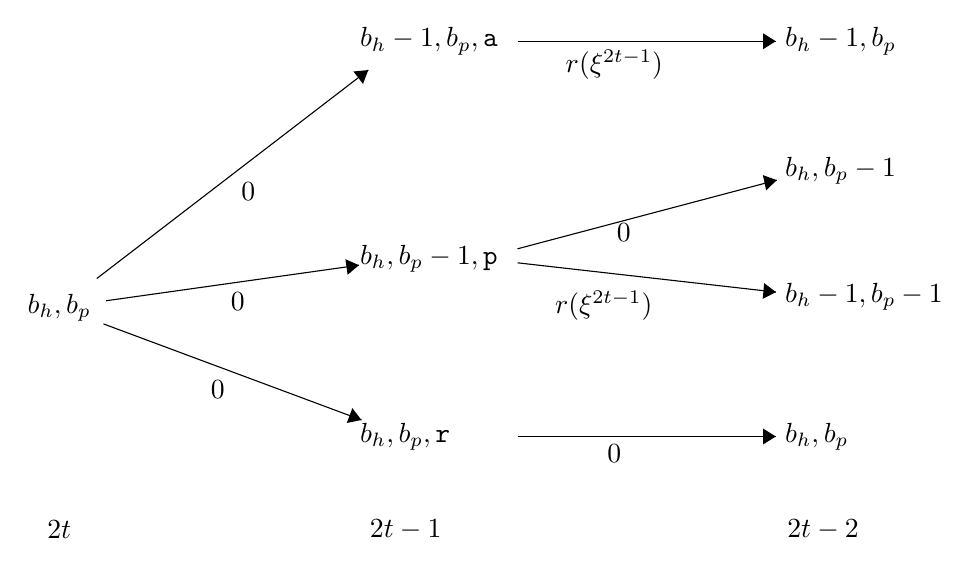
\begin{tikzpicture}[scale=0.2]
\tikzstyle{every node}+=[inner sep=0pt]

\draw (5.9,-25.9) node {$b_h,b_p$};

\draw (5.9,-40) node {$2t$};
\draw (27.9,-40) node {$2t-1$};
\draw (54.4,-40) node {$2t-2$};

\draw (30,-9) node[text width=2cm] {$b_h-1,b_p,\texttt{a}$};
\draw (30,-22.8) node[text width=2cm] {$b_h,b_p-1,\texttt{p}$};
\draw (30,-34.1) node[text width=2cm] {$b_h,b_p,\texttt{r}$};

\draw (57,-9) node[text width=2cm] {$b_h-1,b_p$};
\draw (57,-17.2) node[text width=2cm] {$b_h,b_p-1$};
\draw (57,-34.1) node[text width=2cm] {$b_h,b_p$};
\draw (57,-25.2) node[text width=2cm] {$b_h-1,b_p-1$};


\draw [black] (8.28,-24.07) -- (25.52,-10.83);
\fill [black] (25.52,-10.83) -- (24.58,-10.92) -- (25.19,-11.71);
\draw (17.91,-17.95) node [below] {$0$};
\draw [black] (8.87,-25.48) -- (24.93,-23.22);
\fill [black] (24.93,-23.22) -- (24.07,-22.84) -- (24.21,-23.83);
\draw (17.24,-24.94) node [below] {$0$};
\draw [black] (8.71,-26.95) -- (25.09,-33.05);
\fill [black] (25.09,-33.05) -- (24.51,-32.3) -- (24.16,-33.24);
\draw (15.97,-30.52) node [below] {$0$};

\draw [black] (35,-9) -- (51.4,-9);
\fill [black] (51.4,-9) -- (50.6,-8.5) -- (50.6,-9.5);
\draw (41.15,-9.5) node [below] {$r(\xi^{2t-1})$};
\draw [black] (35,-22.18) -- (51.46,-17.82);
\fill [black] (51.46,-17.82) -- (50.58,-17.5) -- (50.79,-18.47);
\draw (41.75,-20.58) node [below] {$0$};
\draw [black] (35,-23.07) -- (51.41,-24.93);
\fill [black] (51.41,-24.93) -- (50.66,-24.36) -- (50.57,-25.36);
\draw (40.47,-24.83) node [below] {$r(\xi^{2t-1})$};
\draw [black] (35,-34.1) -- (51.4,-34.1);
\fill [black] (51.4,-34.1) -- (50.6,-33.6) -- (50.6,-34.6);
\draw (41.15,-34.6) node [below] {$0$};
\end{tikzpicture}
}
\caption{Transitions for the online probing problem. 
Numbers below the arrows represent the reward of a transition.
At time $2t$ the possible actions are: accept, probe and reject.
At $2t-1$, depending on $\diamond$, we can either accept or reject and $b_h$ may be discounted.
}
\label{fig:probing_states}
\end{figure}




\subsection{Relaxation for Multiple Probing}

The natural relaxation is similar to \cref{eq:probing_relaxation}, but it presents a new challenge.
For binary cases, it was obvious that, if \off wants to probe an arrival, he will always accept it if it is active.
In this case it could be that \off probes $j$ in hope of observing $r_{j2}$ and will reject $r_{j1}$.
We must, therefore, reason about \off's actions at all times, instead of just at even times as before and concluding with structural properties.

Let $\calX\defeq\Rp^{4n}$ be the space for the decision variables.
In \cref{eq:probing_lp} we present a LP which will be the building block for our relaxation.
Note that, by definition, if $t$ is odd, $Z_j(t)=Z_j(t+1)-\In{\xi^{t+1}=j}$.

\begin{equation}\label{eq:probing_lp}
\begin{array}{rrll}
(P[t,Z,b]) \; \max & \multicolumn{3}{l}{\sum_{j,k}r_{jk}(x_{(j,k)a}+q_{jk}x_{ja})} \\
\text{s.t.}& \sum_{j,k}x_{(j,k)a}+\sum_jx_{ja} &\leq b_h  \\
&  \sum_j x_{jp} & \leq b_p   \\
&  x_{ja} +x_{jp} & \leq Z_j(t)  & j\in [n] \\
& x_{(j,k)a} &\leq q_{jk}x_{jp} &  j \in [n],k\in [2]\\ 
& x&\in\calX.
\end{array}
\end{equation}

The LP in \cref{eq:probing_lp} can be interpreted as follows...\todonote

We are ready to parse the relaxation in \cref{eq:probing_relax}.
Recall that a state is of the form $s=(b_h,b_p,\diamond)$ with $\diamond\in \crl{\texttt{a},\texttt{p},\texttt{r},\varnothing}$, where $\diamond=\varnothing$ for even times.
\begin{equation}\label{eq:probing_relax}
\varphi(t,s,\xit) = \left\{ 
\begin{array}{ll}
v(P[t,Z,b]) & \diamond=\varnothing \\ 
v(P[t-1,Z,b]) & \diamond = \texttt{r} \\ 
r_{\xit}+v(P[t-1,Z,b]) & \diamond = \texttt{a} \\ 
\max\crl{r_{\xit}+v(P[t-1,Z,b-e_h]),v(P[t-1,Z,b])} & \diamond = \texttt{p}
\end{array} 
\right.
\end{equation}

\begin{lemma}
Let $\bar X\in\calX$ be a maximizer of $(P[t,Z,b])$ for $t$ even.
Say $\xit=j$, then, at time $t$, \off is satisfied with the following actions:
\begin{enumerate}
\item Accept if $\bar X_{ja}\geq 1$
\item Reject if $\bar X_{ja}+\bar X_{jp}\leq Z_j(t)-1$
\item Probe if $\bar X_{jp}\geq 1$ and then accept $(j,k)$ if $\bar X_{(j,k)a}\geq 1$
\end{enumerate}
\end{lemma}
\begin{proof}
We will show that $\varphi$ satisfies the relaxed Bellman equations, then conclude in virtue of \cref{prop:relaxed_bellman}.
The initial condition follows from the same argument as in \cref{prop:probing_relaxation}.
We are left to show the the probabilistic inequality
\[
\varphi(t,s,\xit) \leq \max_{u\in\U}\crl{R(s,\xit,u)+\E_{\xi^{t-1}}[\varphi(t-1,\Tr(s,\xit,u),\xi^{t-1})|\xit]} \quad \forall \omega\in\calB(t,s).
\]
The set $\calB(t,s)$ is defined as the $\omega\in\Omega$ such that at least one of the conditions (1),(2) or (3) are satisfied.
Observe that, since $t$ is even, the instant reward $R(s,\xit,u)$ is zero.
In cases (1) and (2) is easy to verify the probabilistic inequality.
For case (3) we apply Jensen's Inequality:
\begin{align*}
\varphi(t,s,\xit) &= v(P[t,Z,b]) \\
&= \max\crl{\E[r_{\xi^{t-1}}|\xit]+v(P[t-1,Z,b-e_p-e_h]),v(P[t-1,Z,b-e_p])} \\
&\leq \E_{\xi^{t-1}}[\max\crl{r_{\xit}+v(P[t-1,Z,b-e_h-e_p]),v(P[t-1,Z,b-e_p])}].
\end{align*}
The last term equals $R(s,\xit,u)+\E_{\xi^{t-1}}[\varphi(t-1,s\ominus\texttt{p},\xi^{t-1})|\xit]$ and the proof is complete.
\end{proof}